\documentclass[margin=2mm]{standalone}

\usepackage[
% school,
% simplified
]{pgf-umlcd}

%%%%%%%%%%%%%%%%%%%%%%%%%%%%%%%%%%%%%%%%%%%%%%%%%%%%%%%%%%%%%%%%%
\usepackage{listings}
\usepackage{color}
\definecolor{listinggray}{gray}{0.92}
\lstset{ %
language=[LaTeX]TeX,
breaklines=true,
frame=single,
% frameround=tttt,
basicstyle=\footnotesize\ttfamily,
backgroundcolor=\color{listinggray},
keywordstyle=\color{blue}
}
%%%%%%%%%%%%%%%%%%%%%%%%%%%%%%%%%%%%%%%%%%%%%%%%%%%%%%%%%%%%%%%%%

%%%%%%%%%%%%%%%%%%%%%%%%%%%%%%%%%%%%%%%%%%%%%%%%%%%%%%%%%%%%%%%%%
\usepackage{hyperref}
\hypersetup{
  colorlinks=true,
  linkcolor=blue,
  anchorcolor=black,
  citecolor=olive,
  filecolor=magenta,
  menucolor=red,
  urlcolor=blue
}
%%%%%%%%%%%%%%%%%%%%%%%%%%%%%%%%%%%%%%%%%%%%%%%%%%%%%%%%%%%%%%%%%

%\renewcommand{\umltextcolor}{red}
\renewcommand{\umlfillcolor}{black!6}
\renewcommand{\umldrawcolor}{red!60!black}

\begin{document}

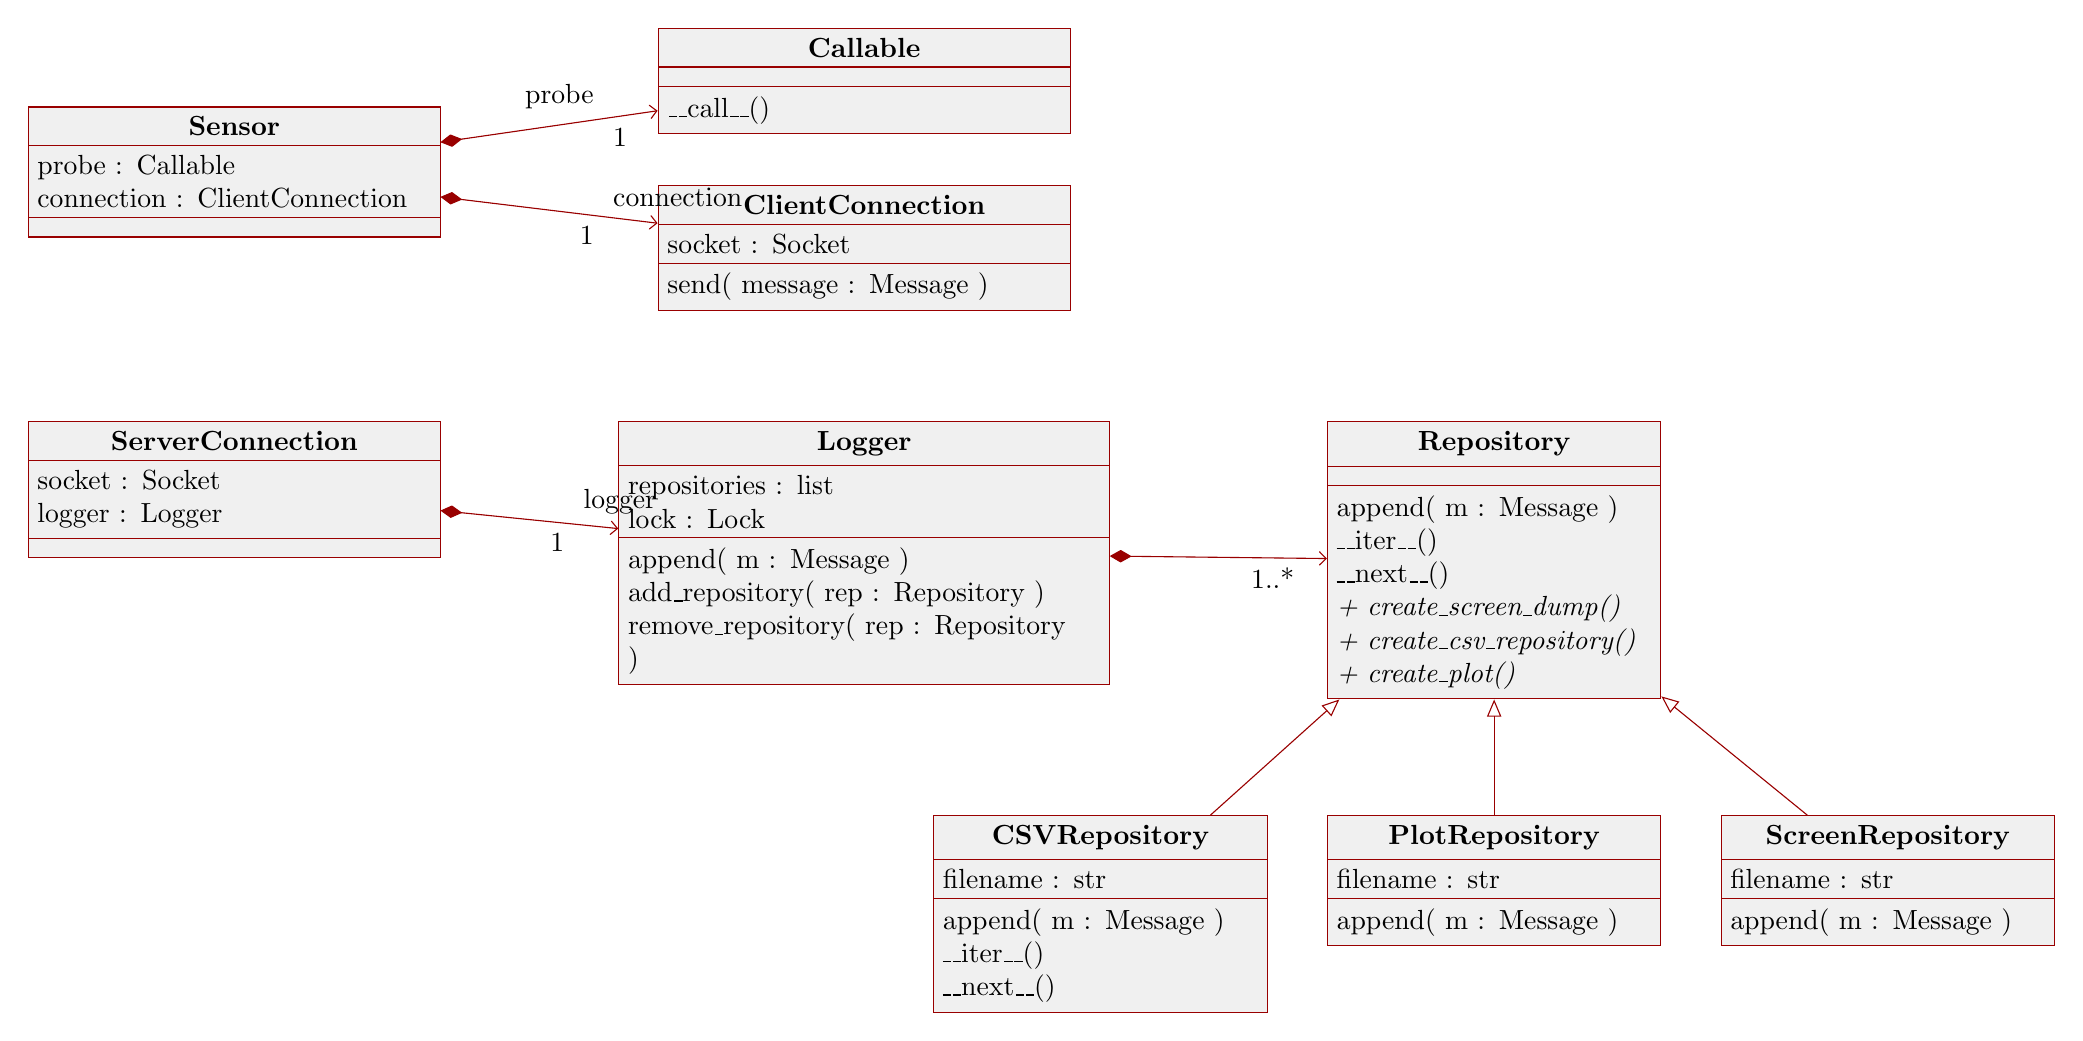
\begin{tikzpicture}[
  % show background grid
  ]
  \begin{class}{Sensor}{0,0}
    \attribute{probe : Callable}
    \attribute{connection : ClientConnection}
  \end{class}

  \begin{class}{Callable}{8, 1}
    \operation{\_\_call\_\_()}
  \end{class}

  \begin{class}{ClientConnection}{8,-1}
    \attribute{socket : Socket}
    \operation{send( message : Message )}
  \end{class}

  \composition{Sensor}{probe}{1}{Callable}
  \composition{Sensor}{connection}{1}{ClientConnection}


  \begin{class}{ServerConnection}{0,-4}
    \attribute{socket : Socket}
    \attribute{logger : Logger}
    
  \end{class}

  \begin{class}[text width = 6cm]{Logger}{8,-4}
    \attribute{repositories : list}
    \attribute{lock : Lock}
    \operation{append( m : Message )}
    \operation{add\_repository( rep : Repository )}
    \operation{remove\_repository( rep : Repository )}
    
  \end{class}

  \composition{ServerConnection}{logger}{1}{Logger}

  \begin{class}[text width = 4cm]{Repository}{16,-4}
    \operation{append( m : Message )}
    \operation{\_\_iter\_\_()}
    \operation{\_\_next\_\_()}
    \operation[0]{+ create\_screen\_dump()}
    \operation[0]{+ create\_csv\_repository()}
    \operation[0]{+ create\_plot()}
  \end{class}


  \composition{Logger}{}{1..*}{Repository}

  \begin{class}[text width=4cm]{CSVRepository}{11,-9}
    \inherit{Repository}
    \attribute{filename : str}
    \operation{append( m : Message )}
    \operation{\_\_iter\_\_()}
    \operation{\_\_next\_\_()}
  \end{class}

  
  \begin{class}[text width=4cm]{ScreenRepository}{21,-9}
    \inherit{Repository}
    \attribute{filename : str}
    \operation{append( m : Message )}
  \end{class}

    \begin{class}[text width=4cm]{PlotRepository}{16,-9}
      \inherit{Repository}
    \attribute{filename : str}
    \operation{append( m : Message )}
  \end{class}
  

\end{tikzpicture}
\end{document}
